\chapter{HPC projects on Twitter} \label{HPC_projects_on_Twitter}
As shown in chapter \ref{FET_projects_and_social_media}, Twitter is the most used social media among FET projects. In particular, roughly 80\% of the HPC projects (17 out of 22) have created a profile on Twitter. This percentage is larger than the corresponding value calculated for the other FET projects. Nevertheless, the result is insufficient to determine how active HPC projects are on Twitter. 

An analysis of the Twitter HPC profiles was performed to assess their activity and influence. The results were integrated by a further analysis, based on the monitoring of the mentions of HPC projects on Twitter over a period of three and a half months. The goal of this second analysis was to estimate the virality of the conversations on the considered projects.  

Both analyses are described in this chapter. Section \ref{Overall_activity} provides an overview of the past activity of the HPC Twitter profiles. Section \ref{Most_influential_projects} identifies the most influential HPC projects. Section \ref{Mentions_of_HPC_profiles} describes the monitoring of the mentions of HPC projects. Section \ref{Projects_with_most_viral_mentions} ranks HPC project in order of virality of their mentions. 

\section{Overall activity} \label{Overall_activity}
\afterpage{
 \clearpage %Flush earlier floats (otherwise order might not be correct)
 \thispagestyle{empty} %empty page style
   \begin{landscape}
   %\begin{table}[htb]
   \begin{table}
   %\begin{adjustwidth}{-1.5cm}{}
   %\begin{adjustwidth}{-1.0cm}{}
   {\tiny
    \begin{tabular}{*{8}{c}} 
      \hline 
  	  \hline
       Project & Date of first tweet & Tweets & Tweets per day & Tweets retweeted & Times per retweeted tweet & Links per tweet & Hashtags per tweet \\ 
       \hline
       \hline
       ALLScale & 26/05/2016 & 39 & 0.08 & 15\% & 1.67 & 0.72 & 0.38 \\
       ANTAREX & 25/09/2015 & 24 & 0.03 & 37\% & 1.56 & 0.63 & 0.04 \\
       COMPAT & 01/10/2015 & 122 & 0.16 & 7\% & 1.63 & 0.30 & 0.05 \\
       DEEP-EST & 19/05/2014 & 900 & 0.72 & 40\% & 2.08 & 0.52 & 1.59 \\
       ECOSCALE & 17/10/2015 & 19 & 0.03 & 21\% & 1.25 & 0.26 & 0.00 \\
       EuroLab-4-HPC & - & 0 & 0 & 0\% & 0 & 0 & 0 \\
       ExaFLOW & 27/10/2015 & 389 & 0.54 & 24\% & 1.63 & 0.62 & 0.97 \\
       ExaNeSt & 29/11/2015 & 1 059 & 1.54 & 13\% & 1.38 & 0.46 & 0.06 \\
       ExaNoDe & 20/06/2017 & 38 & 0.32 & 13\% & 2.60 & 0.21 & 0.03 \\
       EXDCI & 30/03/2016 & 864 & 1.53 & 16\% & 2.90 & 0.20 & 0.23 \\
       EXTRA & 06/10/2015 & 4 & 0.01 & 0\% & 0 & 0.25 & 0.25 \\
       INTERTWINE & 28/11/2016 & 99 & 0.31 & 52\% & 2.18 & 0.77 & 0.79 \\
       MANGO & 03/12/2015 & 32 & 0.05 & 44\% & 1.93 & 0.38 & 0.38 \\
       Mont-Blanc 3 & 06/02/2012 & 2 506 & 1.21 & 24\% & 2.68 & 0.32 & 0.50 \\
       NEXTGenIO & 30/09/2015 & 211 & 0.28 & 24\% & 3.02 & 0.14 & 0.52 \\
       READEX & 13/10/2015 & 29 & 0.04 & 69\% & 1.60 & 0.62 & 1.03 \\
       SAGE & 30/09/2015 & 92 & 0.12 & 33\% & 1.77 & 0.20 & 0.07 \\ 
       FET & 07/01/2016 & 3 199 & 4.94 & 32\% & 4.46 & 0.42 & 0.92 \\
       \hline
       \hline
    \end{tabular}
   }     
   \caption{Statistics collected from the Twitter accounts of the HPC projects funded in Horizon 2020. The data were collected from the date of the projects' first tweet to 14 October 2017. Tweets per day is the average number of tweets posted each day. Tweets retweeted corresponds to the fraction of the project's tweets which have been retweeted by other accounts. Times per retweeted tweet refers to the average number of times a retweeted post has been retweeted. The last two columns report the average number of links and hashtags per project's tweet. The statistics collected for the Twitter profiles used by the DEEP-EST and Mont-Blanc 3 projects include the activities of the previous phases of these initiatives as well, namely the DEEP and DEEP-ER projects and the Mont-Blanc and Mont-Blanc 2 actions. The EuroLab-4-HPC project has posted no tweets since the creation of the account. The last row refers to the @fet\textunderscore eu profile of the FET funding programme. For this account, the statistics are limited to the maximum number of most recent tweets returned by Twitter (3200). Data were collected with the Twitter Analytics Tool Twitonomy.} \label{HPC_Twitter_activity}
   %\end{adjustwidth} 
   \end{table}
   \end{landscape}
 \clearpage
}

The past activity of the Twitter accounts of HPC projects was analysed with the Twitter Analytics Tool Twitonomy \cite{Twitonomy}. For each profile, data were collected from the project's first Tweet to 14 October 2017. The statistics extracted for each project are listed in table \ref{HPC_Twitter_activity}. The results of the analysis are outlined in the following subsections\footnote{Hereafter it must be borne in mind that the Twitter profiles used by the DEEP-EST and Mont-Blanc 3 projects have been created for the previous stages of these initiatives: @DEEPprojects was also used for the DEEP and DEEP-ER projects, @MontBlanc\textunderscore Eu for Mont-Blanc and Mont-Blanc 2, see \cite{DEEPprojects,MontBlanc}. Hence, the statistics relative to DEEP-EST and Mont-Blanc 3 have been calculated over the whole activity of the respective accounts.}.

\begin{figure}
 \centering
 \begin{subfigure}[t]{0.95\textwidth}
   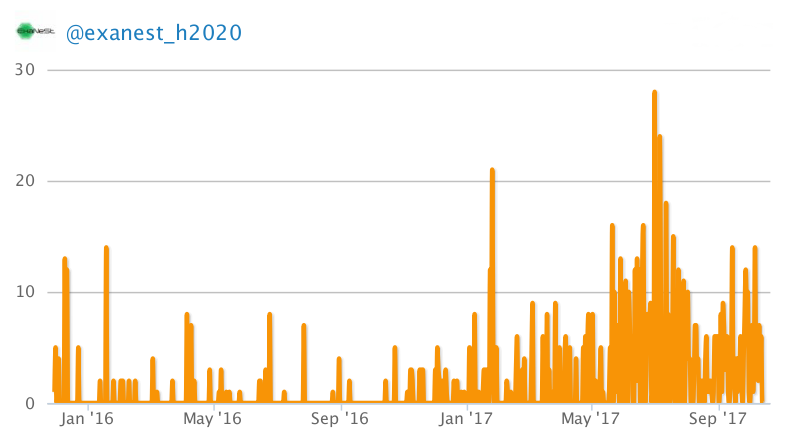
\includegraphics[width=1\linewidth]{Images/Tweets_Exanest.png}
   \caption{} 
 \end{subfigure}

\begin{subfigure}[t]{0.95\textwidth}
   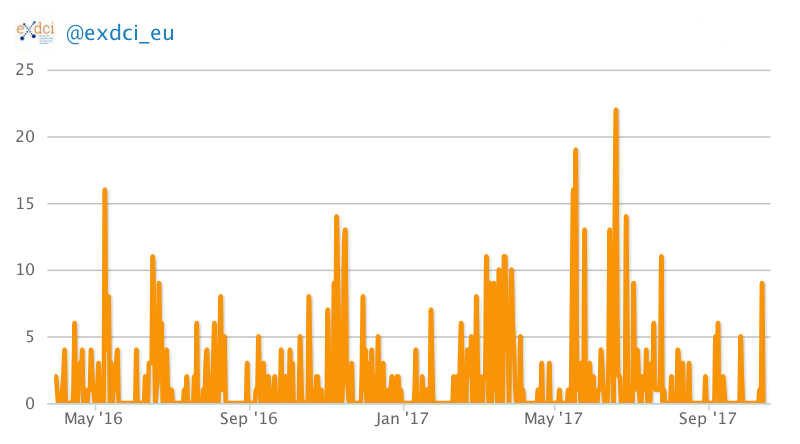
\includegraphics[width=1\linewidth]{Images/Tweets_Exdci.png}
   \caption{}
 \end{subfigure}
 \caption{(a) Time distribution of the number of tweets posted by ExaNeSt, the HPC project with the largest average number of tweets per day (1.54) as of 14 October 2017. (b) As for (a) but for EXDCI, the HPC project with the second largest average number of tweets per day (1.53). The plots were generated with the Twitter Analytics Tool Twitonomy.} 
 \label{Tweets_Exanest-Exdci}
\end{figure}

\begin{figure}
 \centering
 \begin{subfigure}[t]{0.95\textwidth}
   \includegraphics[width=1\linewidth]{Images/Tweets_Montblanc.png}
   \caption{} 
 \end{subfigure}

 \begin{subfigure}[t]{0.95\textwidth}
   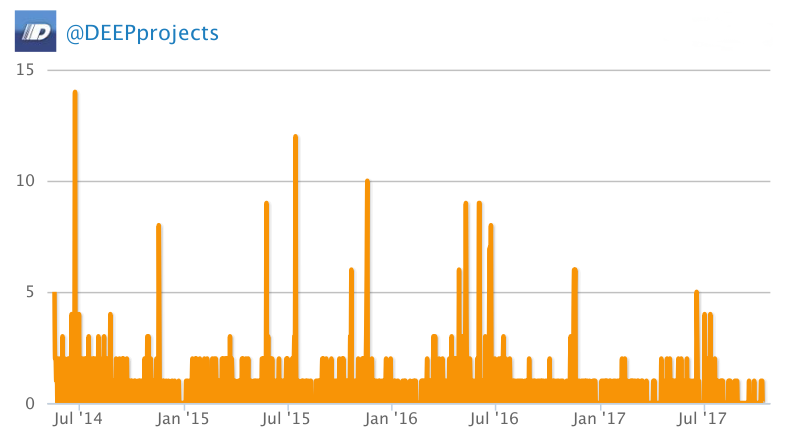
\includegraphics[width=1\linewidth]{Images/Tweets_Deepest.png}
   \caption{}
 \end{subfigure}
 \caption{(a) Time distribution of the number of tweets posted on the profile used by Mont-Blanc 3, the HPC account with the third largest average number of tweets per day (1.21) as of 14 October 2017. (b) As for (a) but for the profile used by DEEP-EST, the HPC account with the fourth largest average number of tweets per day (0.72). The plots were generated with the Twitter Analytics Tool Twitonomy.} 
 \label{Tweets_Montblanc-Deepest}
\end{figure}

\subsubsection{Tweets per day}
Out of the seventeen considered HPC Twitter profiles, three have an average tweeting rate larger than one post per day. The time distribution of the tweets of the accounts with the highest average rates are shown in figures \ref{Tweets_Exanest-Exdci} and \ref{Tweets_Montblanc-Deepest}. The tweeting rate is lower than one every second day for twelve profiles. One project has posted no tweets since the creation of the account. 

The median of the projects' rates is 0.16 tweets/day. This corresponds to roughly 5 posts per month. The median was chosen as representative value of the HPC posting rate for its robustness in the presence of outliers, see also section \ref{Budget_impact}.

\subsubsection{Retweets}
The fraction of an account's posts retweeted by others offers an estimate of the effectiveness of the user's  activity on Twitter. The higher the percentage, the more the profile is considered a valuable source of information by the Twitter community. 

The HPC project with the largest fraction of tweets retweeted by other accounts is READEX ($\sim 70\%$). Except for one, all other profiles have a percentage value smaller than 50\%. The median of the fraction of retweeted tweets calculated over all HPC projects is $\sim 25\%$.

The results on the percentage of retweeted posts are integrated by the average number of times such tweets were retweeted by different users. The higher this value, the more the Twitter community finds the profile's tweets worth to be forwarded. 

Table \ref{HPC_Twitter_activity} shows that six projects have an average number of retweet times higher or equal to two, i.e., retweeted posts have been retweeted by typically more than two users. The median calculated over all profiles is $\sim 1.7$.

\subsubsection{Links and hashtags}
Links and hashtags enhance the relevance of a tweet. The higher the average number of links per tweet for a given profile, the more likely the account is a source of information to other users. The higher the average number of hashtags per tweet, the higher the chance that the profile's tweets are found in a search.

As shown in table \ref{HPC_Twitter_activity}, six HPC accounts have an average number of links per tweet higher or equal to 0.5, the value corresponding to one link every second tweet. The median calculated over all HPC accounts is $\sim 0.3$, i.e. roughly one link every third tweet. Three accounts have an average number of hashtags equal or larger than one. The median is 0.25, corresponding to one hashtag every fourth tweet.

\subsubsection{Comparison to the FET Twitter profile}
Table \ref{HPC_Twitter_activity} reports the statistics calculated for the Twitter profile @fet\textunderscore eu of the FET funding programme as well. Data were collected from 7 January 2016. The date was set by the maximum number of most recent tweets returned by Twitter (3200). 

The corresponding average number of tweets per day is roughly thirty times larger than the median calculated for HPC projects. This is probably due to the largest resources available to the FET initiative compared to single HPC projects. Nevertheless, the fraction of retweeted tweets is not significantly larger than the median calculated for the HPC profiles ($\sim 30\%$ vs $\sim 25\%$). The same holds for the average number of links per tweet ($\sim 0.4$ vs $\sim 0.3$). On the contrary, the average number of hashtags is roughly four times larger ($\sim 0.9$ vs 0.25).

\section{Most influential projects} \label{Most_influential_projects}
There are disparate ways to estimate the influence of Twitter profiles. One is based on both \textit{i}) the number of followers, and \textit{ii}) the ratio between the number of followers and the number of accounts followed by the considered profile (following). Influential users are identified by a large community of followers and a high ratio followers/following.

\begin{table}[t]
 \begin{center}
 {\scriptsize
  \begin{tabular}{cccc}
   \hline 
   \hline
   Project & Followers & Following & Followers/Following \\ 
   \hline
   \hline
   ALLScale & 41 & 28 & 1.46 \\
   ANTAREX & 77 & 13 & 5.92 \\
   COMPAT & 131 & 160 & 0.82 \\
   DEEP-EST & 697 & 534 & 1.31 \\
   ECOSCALE & 42 & 1 & 42 \\
   EuroLab-4-HPC & 24 & 2 & 12 \\
   ExaFLOW & 206 & 90 & 2.29 \\
   ExaNeSt & 211 & 261 & 0.81  \\
   ExaNoDe & 52 & 54 & 0.96 \\
   EXDCI & 405 & 169 & 2.40 \\
   EXTRA & 45 & 18 & 2.50\\
   INTERTWINE & 106 & 59 & 1.80 \\
   MANGO & 74 & 46 & 1.61 \\
   Mont-Blanc 3 & 1 420 & 687 & 2.07 \\
   NEXTGenIO & 162 & 44 & 3.86 \\
   READEX & 116 & 55 & 2.11 \\
   SAGE & 122 & 86 & 1.42 \\ 
   FET & 6 499 & 1 612 & 4.03 \\
   \hline
   \hline
  \end{tabular}
 } 
 \end{center} 
 \caption{Number of followers and followed accounts (following) on Twitter of the HPC projects as of 14 October 2017. Influential profiles are identified by high numbers of followers and high values of the ratio between followers and following. The last row refers to the @fet\textunderscore eu profile of the FET funding programme. Data were collected with the Twitter Analytics Tool Twitonomy.}
\label{HPC_influence_table} 
\end{table}

Table \ref{HPC_influence_table} lists the number of followers and following for each HPC project, together with the ratio followers/following. Data were collected on 14 October 2017 with the Twitonomy application. The medians of the number of followers and of the values followers/following are equal to 116 and 2.07, respectively. 

\begin{figure}[!t] 
 \begin{center}
 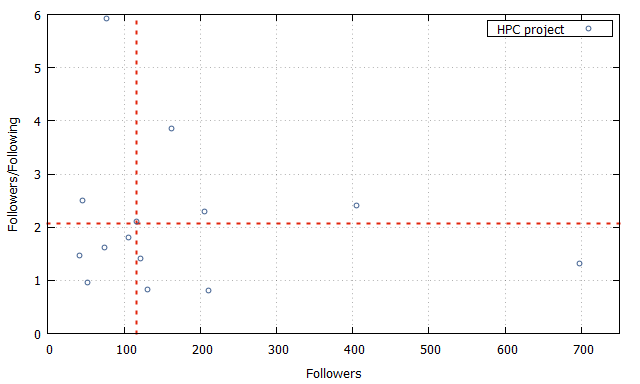
\includegraphics[scale=0.5]{Images/HPC_influence.png}
 \caption{Distribution of HPC projects as a function of the number of followers and of the ratio between followers and followed accounts (following) on Twitter. The dashed lines identify the medians of the numbers of followers and of the ratios followers/following calculated over the HPC profiles. The most influential projects are located in the upper right quarter (high number of followers and high values of followers/following). For the sake of clarity, the figure shows the followers and followers/following ranges up to 750 and 6, respectively. The following projects were used to calculated the medians but lie outside the plotted ranges: ECOSCALE (42 followers and follower/following equal to 42), EuroLab-4-HPC (24 and 12) and Mont-Blanc 3 (1420 and 2.07). Data were collected on 14 October 2017 with the Twitter Analytics Tool Twitonomy.}
 \label{HPC_influence_plot}
 \end{center}
\end{figure}

To identify the most influential profiles among HPC projects, the following analysis was performed. First, projects were distributed on a plane as a function of the number of followers and of the ratio followers/following, see figure \ref{HPC_influence_plot}. Second, the plane was divided into four regions by drawing the lines corresponding to the aforementioned medians of the number of followers and of the values followers/following. The most influential HPC projects fall in the quarter of the plane identified by the conditions that the number of followers is larger than 116 and the ratio followers/following is larger than 2.07.

By following this procedure, the most influential projects were found to be ExaFLOW (206, 2.29), EXDCI (405, 2.40), Mont-Blanc 3 (1420, 2.07) and NEXTGenIO (162, 3.86). The READEX profile (116, 2.11) is representative of the influence of HPC projects, as its values lie very close to the calculated medians. For comparison, the @fet\textunderscore eu profile of the FET funding programme has 6499 followers and a ratio followers/following equal to 4.03.

\section{Mentions of HPC profiles} \label{Mentions_of_HPC_profiles} 
Another approach to estimate the influence of HPC projects on Twitter consists of monitoring the mentions of their accounts (i.e., mentions of @AllScaleEurope, @antarex\textunderscore project etc.). The monitoring activity was conducted from 1 July to 12 October 2017 with the Twitter Analytics Tool NUVI \cite{NUVI}.  

\begin{figure}[!t] 
 \begin{center}
 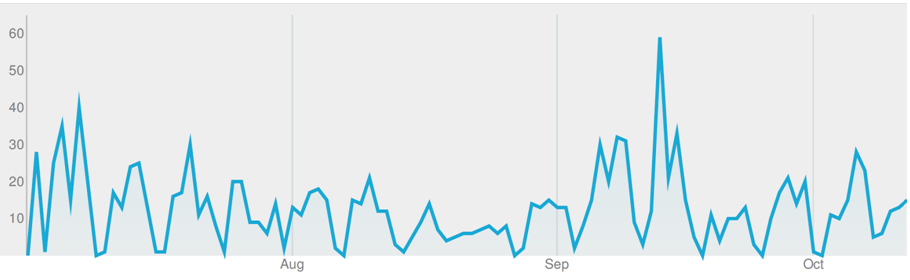
\includegraphics[scale=0.47]{Images/NUVI_time_distribution.png}
 \caption{Time distribution of the mentions of HPC profiles on Twitter between 1 July and 12 October 2017. The plot was created with the Twitter Analytics Tool NUVI.}
 \label{NUVI_time_distribution}
 \end{center}
\end{figure}

\subsubsection{Overview}
Monitored mentions sum up to 1323. The time distribution of the mentions is shown in figure \ref{NUVI_time_distribution}. The conversation peak happened on 12 September 2017 (59 mentions). During the peak, the most frequently used keywords were \textit{filippo mantovani}, \textit{workshop}, \textit{server cpu}, \textit{prototype} and \textit{processors}. An overview of the topics discussed in the monitored mentions is provided in figure \ref{HPC_word_burst}. The figure is based on the 1005 mentions which came across 485 major categories over the monitored time. The list of the most shared words is in table \ref{Most_shared_words}.

\begin{table}[t]
 \begin{center}
 %{\scriptsize
  \begin{tabular}{cccc}
   \hline 
   \hline
   Shared word & Mentions & Fraction of total mentions \\ 
   \hline
   \hline
   amp & 22 & 2.2\% \\
   project & 18 & 1.8\% \\
   supercomputer & 16 & 1.6\% \\
   application & 15 & 1.5\% \\
   etp4h & 14 & 1.4\% \\
   compute & 11 & 1.1\% \\
   \hline
   \hline
  \end{tabular}
 %} 
 \end{center} 
 \caption{List of the most shared words in the 1005 mentions of the HPC profiles which came across 485 of the major categories considered by the Twitter Analytics Tool NUVI. These mentions are a subset of the 1323 mentions monitored with NUVI between 1 July and 12 October 2017. The second and third columns report the amount of mentions in which the considered word was shared and the percentage of the total mentions. }
\label{Most_shared_words} 
\end{table}

\subsubsection{Virality of the mentions}
Reach and spread together give an estimate of the potential audience which came across with the tweeted content. The reach is calculated as the sum of the followers of the accounts which mentioned the analysed keyword. The spread is defined as the sum of the followers of the accounts which retweeted or shared the posts with the mention. Figure \ref{HPC_Most_reach_spread_popular} shows the mentions with the largest reach and spread, as well as the most popular one.

Out of the 1323 monitored mentions, 637 were original posts. These had the combined potential of reaching an audience of 172720 users. A total amount of 686 reshares was made by 116 unique profiles. The reshares spread the mentions to 233974 users.

%\begin{figure}[H]
\begin{figure}[!t] 
 \begin{center}
 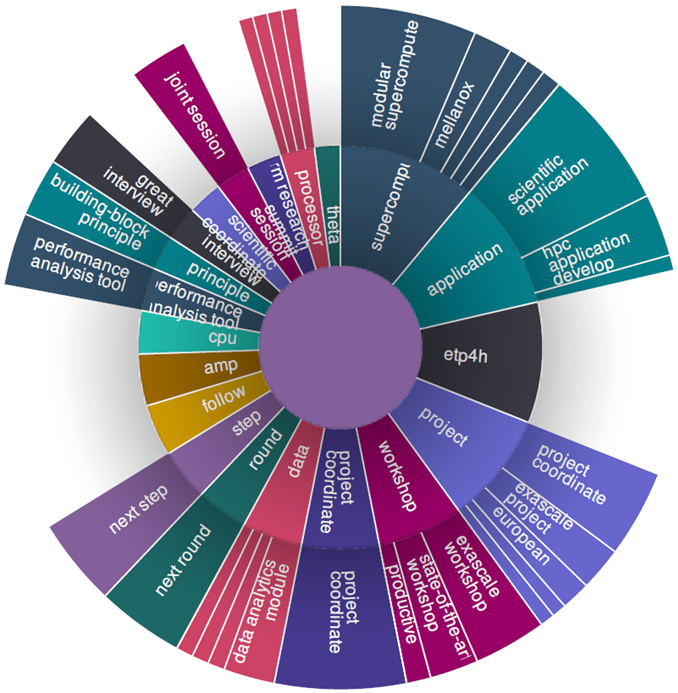
\includegraphics[scale=0.64]{Images/HPC_word_burst.png}
 \caption{Word burst of the mentions of HPC profiles monitored between 1 July and 12 October 2017 on Twitter. The figure is based on the 1005 mentions (out of 1323) which triggered 485 major categories. The analysis was performed with the Twitter Analytics Tool NUVI.}
 \label{HPC_word_burst}
 \end{center}
\end{figure}

The ratio between spread and reach defines the viral coefficient. This is equal to 1.4 for the monitored mentions and over the considered period, see figure \ref{HPC_viral_coefficient}. As the viral coefficient is larger than one, monitored mentions can be considered extremely viral. 

\begin{figure}[!t] 
 \begin{center}
 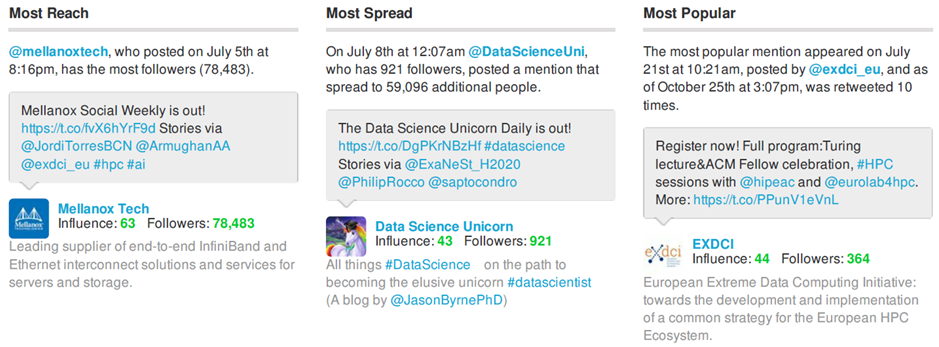
\includegraphics[scale=0.47]{Images/HPC_Most_reach_spread_popular.png}
 \caption{Three of the 1323 mentions of HPC projects on Twitter monitored between 1 July and 12 October 2017. The posts are the mentions with the most reach, the most spread and the most popular one. Data were collected with the Twitter Analytics Tool NUVI.}
 \label{HPC_Most_reach_spread_popular}
 \end{center}
\end{figure}

\begin{figure}[!t] 
 \begin{center}
 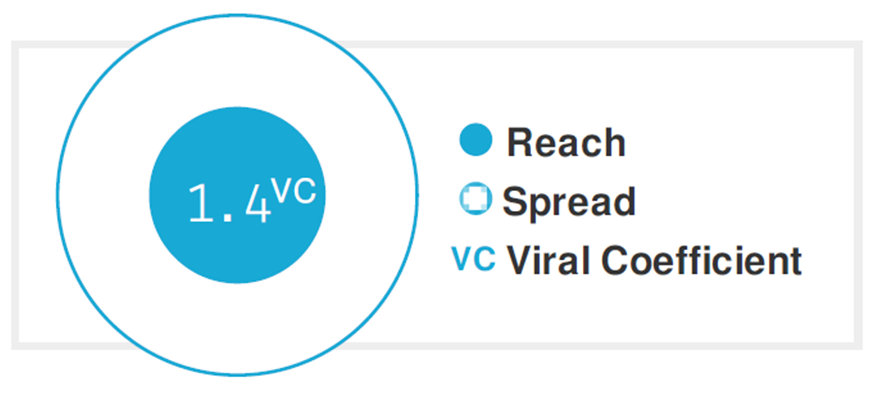
\includegraphics[scale=0.3]{Images/HPC_viral_coefficient.png}
 \caption{Pictorial comparison of the reach (172720 users) and spread (233974 users) of the mentions of HPC projects on Twitter between 1 July and 12 October 2017. The viral coefficient is defined as the ratio between spread and reach. Data were collected with the Twitter Analytics Tool NUVI.}
 \label{HPC_viral_coefficient}
 \end{center}
\end{figure}

\section{Projects with most viral mentions} \label{Projects_with_most_viral_mentions}
Results in section \ref{Mentions_of_HPC_profiles} refer to the whole set of mentions of HPC projects monitored over the considered weeks. The data breakdown for each single project is reported in table \ref{HPC_viral_coefficients}. It is worth noting that the values of reach, spread and viral coefficient vary significantly among HPC projects. The medians of the three variables are 4056, 4836 and 0.7, respectively.     
 
\begin{table}[t]
 \begin{center}
 {\scriptsize
  \begin{tabular}{cccc}
   \hline 
   \hline
   Project & Reach & Spread & Viral coefficient \\ 
   \hline
   \hline
   ALLScale & 48 & 0 & 0.0 \\
   ANTAREX & 202 & 9 & 0.0 \\
   COMPAT & 13 286 & 112 & 0.0 \\
   DEEP-EST & 11 759 & 6 988 & 0.6 \\
   ECOSCALE & 55 & 2 268 & 41.2 \\
   EuroLab-4-HPC & 2 135 & 14 679 & 6.9 \\
   ExaFLOW & 18 366 & 28 311 & 1.5 \\
   ExaNeSt & 18 109 & 62 259 & 3.4  \\
   ExaNoDe & 6 559 & 4 470 & 0.7 \\
   EXDCI & 111 534 & 23 082 & 0.2 \\
   EXTRA & 216 & 24 & 0.1 \\
   INTERTWINE & 7 436 & 6 673 & 0.9 \\
   MANGO & 1 360 & 162 & 0.1 \\
   Mont-Blanc 3 & 30 362 & 58 782 & 1.9 \\
   NEXTGenIO & 4 056 & 53 838 & 13.5 \\
   READEX & 117 & 0 & 0.0 \\
   SAGE & 1 537 & 4 836 & 3.1 \\ 
   \hline
   \hline
  \end{tabular}
 } 
 \end{center} 
 \caption{Reach, spread and viral coefficient of the mentions of each HPC project on Twitter between 1 July and 12 October 2017. The viral coefficient is defined as the ratio between spread and reach. Data were collected with the Twitter Analytics Tool NUVI.}
\label{HPC_viral_coefficients} 
\end{table}

Seven out of seventeen projects have been mentioned in viral conversations (i.e., with viral coefficient larger than one). The projects with the largest viral coefficients are ECOSCALE (41.2), NEXTGenIO (13.5) and EuroLab-4-HPC (6.9). It is worth noting the following: \textit{i}) the large viral coefficient of ECOSCALE originates from the project's low reach; \textit{ii}) EuroLab-4-HPC is mentioned in viral posts although it had posted no tweets by the time of writing, see table \ref{HPC_Twitter_activity}; \textit{iii}) with the exception of EXDCI, the most influential projects identified in section \ref{Most_influential_projects} are all mentioned in viral conversations.

\section{Chapter summary}
In this chapter, the following items have been discussed:

\begin{enumerate}
 \item The activity of HPC projects on Twitter varies from roughly one tweet every three months and three tweets every second day. The median calculated over all HPC Twitter profiles is approximately one tweet per week. HPC projects perform well in terms of profile's tweets retweeted by other users and shared links. The medians of the two statistics are comparable to the corresponding values calculated for the Twitter account of the FET funding programme.
 \item The most influential HPC projects on Twitter were found to be ExaFLOW, EXDCI, Mont-Blanc 3 and NEXTGenIO. In general, HPC influential initiatives are identified by a number of followers and a ratio followers/following larger than $\sim 100$ and $\sim 2$, respectively. 
 \item The mentions of HPC projects on Twitter were found to be viral over a period of three and a half months. The result indicates that the Twitter community interested in FET HPC initiatives is large. This supports the decision of the vast majority of HPC projects to consider Twitter for their communication campaigns.
 \item In general, the most influential HPC projects are also those mentioned in the most viral monitored conversations.    
\end{enumerate}  